\documentclass[eng,openany]{mgr}
\usepackage{listings}
\usepackage[english]{babel}
\usepackage{graphicx}
\usepackage{hyperref}
\usepackage{tabularx,colortbl} 
\usepackage{rotating}
\usepackage[utf8]{inputenc} 
\setlength\parindent{24pt}
\usepackage[parfill]{parskip}
\usepackage[table,kernelfbox,hyperref]{xcolor}
\usepackage{fancyhdr}
\usepackage{gauss}
%\usepackage[colorinlistoftodos]{todonotes}

\hypersetup{colorlinks=true}
\hypersetup{xurlbordercolor=red!70!black}
\hypersetup{xlinkbordercolor=blue!70!black}
\hypersetup{linkcolor=blue!60!black}
\hypersetup{urlcolor=red!50!black}
\hypersetup{citecolor=green!30!black}
\rfoot{Page \thepage}
\renewcommand\lstlistlistingname{List of Listings}
\newcommand{\linia}{\rule{\linewidth}{0.4mm}}

\definecolor{listlightgray}{gray}{0.97}

\newcommand{\lstsetmylst} {
\lstset{frame = tb,
breaklines=true,
framerule = 0.25pt,
float,
fontadjust,
backgroundcolor={\color{listlightgray}},
basicstyle = {\ttfamily\footnotesize},
identifierstyle = {\ttfamily},
stringstyle = {\ttfamily},
showstringspaces = false,
showtabs = false,
numbers = left,
numbersep = 6pt,
tabsize = 4,
language=C,
floatplacement=!h
}
}

\newcommand{\lstsetatc} {
\lstset{frame = tb,
breaklines=true,
framerule = 0.25pt,
float,
fontadjust,
backgroundcolor={\color{listlightgray}},
basicstyle = {\ttfamily\footnotesize},
keywordstyle = {\ttfamily\color{listkeyword}\textbf},
identifierstyle = {\ttfamily},
commentstyle = {\ttfamily\color{listcomment}\textit},
stringstyle = {\ttfamily},
showstringspaces = false,
showtabs = false,
numbers = left,
numbersep = 6pt,
numberstyle={\ttfamily\color{listnumbers}},
tabsize = 4,
language=C,
floatplacement=!h
}
}

\newcommand{\lstsetatbashnum} {
\lstset{frame = tb,
breaklines=true,
framerule = 0.25pt,
aboveskip=2ex,
float,
fontadjust,
backgroundcolor={\color{listlightgray}},
basicstyle = {\ttfamily\footnotesize},
keywordstyle = {\ttfamily\color{listkeyword}\textbf},
identifierstyle = {\ttfamily},
commentstyle = {\ttfamily\color{listcomment}\textit},
stringstyle = {\ttfamily},
showstringspaces = false,
showtabs = false,
numbers = left,
numbersep = 6pt,
numberstyle={\ttfamily\color{listnumbers}},
tabsize = 4,
language=bash,
floatplacement=!h
}
}
\lstsetmylst
\author{Jaroslaw M. Szumega}
\title{}
\engtitle{}
\supervisor{Rafal Zdunek, D.Sc, K-4/W4}
\field{Electronics}
\specialisation{Advanced Applied Electronics}
\date{06.04.2017}
\begin{document}
\selectlanguage{english}
\maketitle
\tableofcontents
\chapter{Solution to the given problems}
The solutions below are the requested numerical results of requested problems as well as the execution time's comparison between different algorithms. To ensure proper timings, all measurements are made for one thousands rounds/repetition -- it will help to reduce the impact of setting up the Octave engine and other overheads.
\begin{figure}[h]
	\centering
	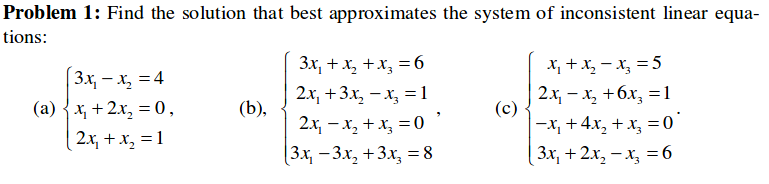
\includegraphics[width=0.6\linewidth]{screenshot001}
	\label{fig:screenshot001}
\end{figure}
\\Each system was solved using set of algorithms dedicated for solving Least Squares problem: there was LS approximation, solving LS using Singular Vector Decomposition (SVD) or QR factorization. In addition the first system is solved also by linear regression.
\begin{lstlisting}
Matrix A
Classical LS
	time =  0.12578
SVD LS
	time =  0.78760
QR LS
	time =  0.061208
regression
	time =  0.087359

Matrix B
Classical LS
	time =  0.043440
SVD LS
	time =  0.86493
QR LS
	time =  0.059717

Matrix C
Classical LS
	time =  0.041433
SVD LS
	time =  0.81831
QR LS
	time =  0.057312
\end{lstlisting}
\begin{figure}[h]
\centering
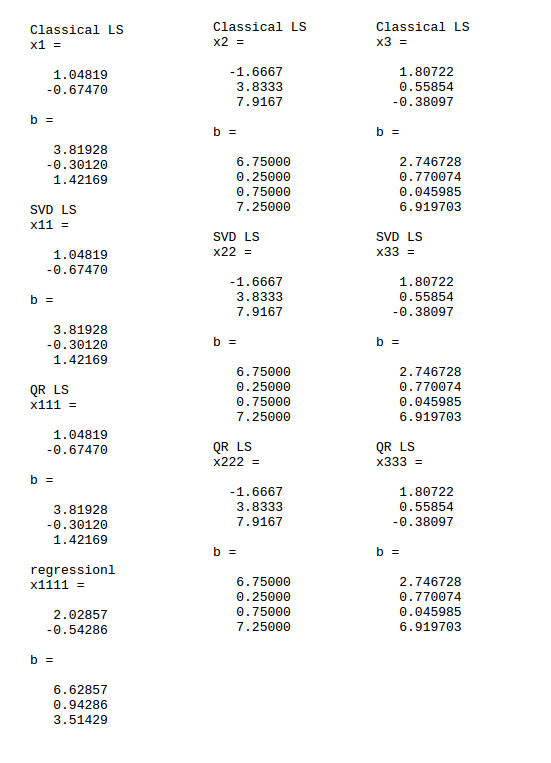
\includegraphics[width=0.7\linewidth]{screenshot003}
\caption{Calculations results. Also verification in form b = Ax}
\label{fig:screenshot003}
\end{figure}
\hspace{40pt}
\newpage
\begin{figure}[h]
\centering
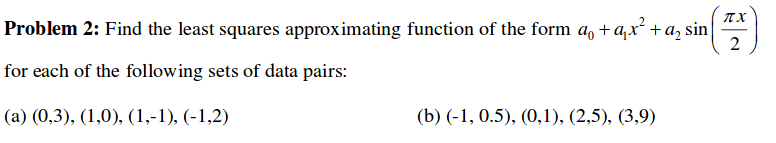
\includegraphics[width=0.7\linewidth]{screenshot004}
\label{fig:screenshot004}
\end{figure}

The selected systems was written in the form of matrices. In Octave code it is like this:
\begin{lstlisting}
A1= [1 0 sin(3.14*0/2);
1 1 sin(3.14*1/2);
1 1 sin(3.14*1/2);
1 1 sin(3.14*(-1)/2); ]

b1 = [3; 0; -1; 2]


# b)
A2 = [1 1 sin(3.14*(-1)/2);
1 0 sin(3.14*0/2);
1 4 sin(3.14*2/2);
1 9 sin(3.14*3/2); ]

b2 = [0.5; 1; 5; 9]
\end{lstlisting}
Then the algorithms were applied to get the solution.

\begin{figure}[h]
	\centering
	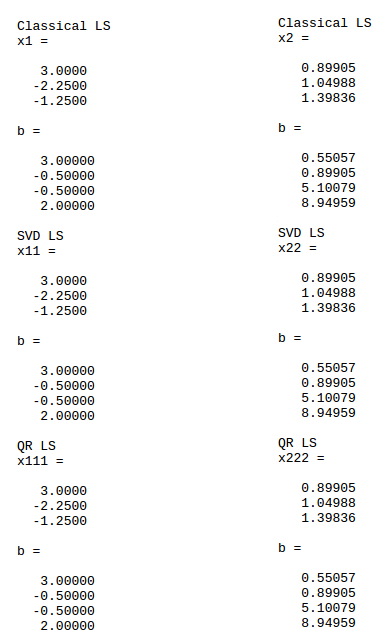
\includegraphics[width=0.5\linewidth]{screenshot005}
	\label{fig:screenshot005}
\end{figure}

As the picture shows, the calculated coefficients gives quite a good approximation, when using them in computing the "b" vector.

The listing below show also timings of selected algorithms:

\begin{lstlisting}

Case A:

Classical LS
	time =  0.050778
SVD LS
	time =  0.73374
QR LS
	time =  0.051985


Case B:

Classical LS
	time =  0.034670
SVD LS
	time =  0.71804
QR LS
	time =  0.051468
\end{lstlisting}
\newpage
\begin{figure}[h]
\centering
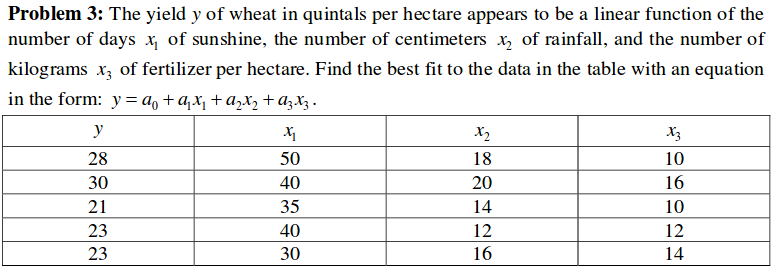
\includegraphics[width=0.7\linewidth]{screenshot006}
\label{fig:screenshot006}
\end{figure}

The problem mentioned above should be presented in form of matrix:
\begin{figure}[h]
\centering
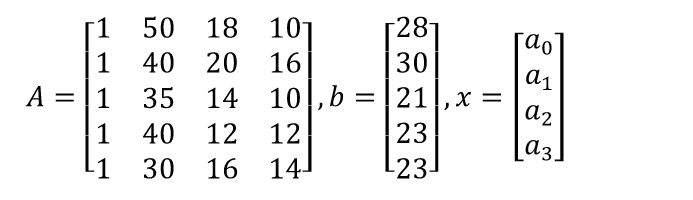
\includegraphics[width=0.5\linewidth]{screenshot007}
\label{fig:screenshot007}
\end{figure}
Once again, the set of selected algorithms will be used. This time there also will be selected the Thikonov regularization.

\begin{figure}[h]
\centering
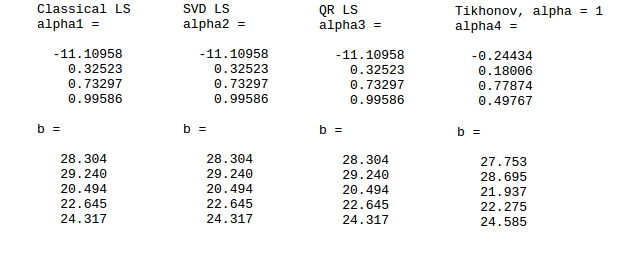
\includegraphics[width=0.7\linewidth]{screenshot008}
\caption{Results.}
\label{fig:screenshot008}
\end{figure}
Looking at \ref{fig:screenshot008} we can see, that all the solutions during the verification give quite good approximation of "b". The first three has exactly the same values and are much better than last algorithm. However, Tikhonov regularization gives the coefficients that stand out of the rest of solutions, but this solution is still correct.

And the timing comparison:
\begin{lstlisting}
Classical LS
time =  0.064596


SVD LS
time =  0.75261


QR LS
time =  0.052665


Gen. Tikhonov, alpha = 1
time =  0.041787
\end{lstlisting}
\newpage
\begin{figure}[h]
\centering
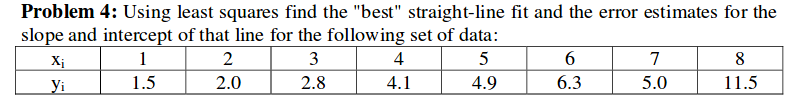
\includegraphics[width=0.7\linewidth]{screenshot009}
\label{fig:screenshot009}
\end{figure}
At first, the problem presented in matrices:
\begin{figure}[h]
\centering
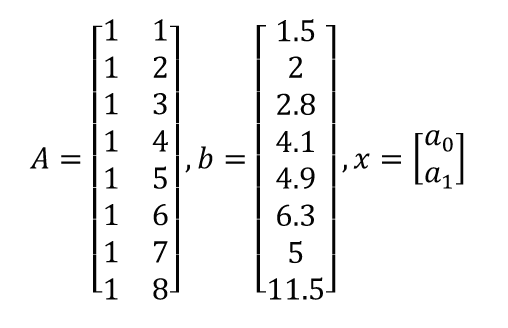
\includegraphics[width=0.35\linewidth]{screenshot010}
\label{fig:screenshot010}
\end{figure}
The results below show the solution computed by different methods. The first three methods are pretty the same answers.
\begin{figure}[h]
\centering
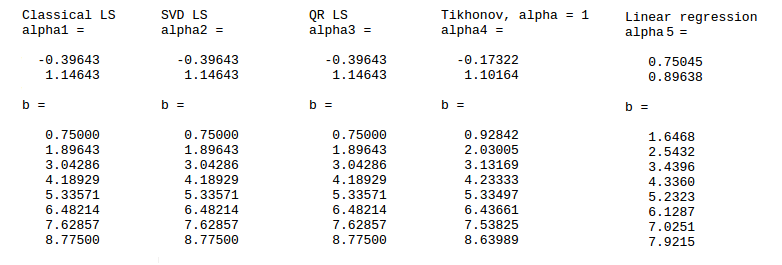
\includegraphics[width=0.8\linewidth]{screenshot011}
\label{fig:screenshot011}
\end{figure}


There were also calculated the timings and the errors of the selected methods:
\begin{lstlisting}
Classical LS
	error =  3.8985
	time =  0.043488
	
SVD LS
	error =  3.8985
	time =  0.72264
	
QR LS
	error =  3.8985
	time =  0.054575
	
Tikhonov, alpha = 1
	error =  3.9098
	time =  0.057088
	
Linear regression
	error =  4.9385
	time =  0.071316
\end{lstlisting}
As it turned out, the best algorithm considering both time and error is the classical LS fitting. The SVD and QR based algorithms gave the same solution, but were slower (especially SVD, which also in previous tasks was slow).
\newpage

\begin{figure}[h]
\centering
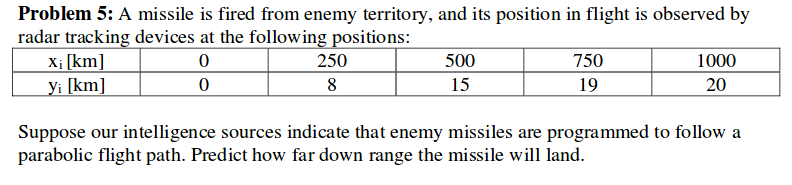
\includegraphics[width=0.7\linewidth]{screenshot012}
\label{fig:screenshot012}
\end{figure}
In this case, as the position of the missle can be described using parabola, so here we are considering the polynomial of second degree.
\begin{figure}[h]
\centering
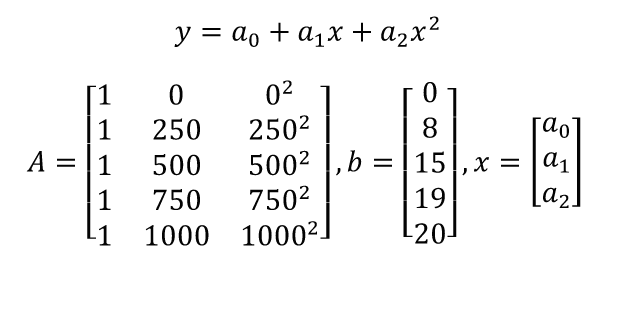
\includegraphics[width=0.4\linewidth]{screenshot014}
\label{fig:screenshot014}
\end{figure}

Using different methods, the following solutions were obtained:
\begin{figure}[h]
\centering
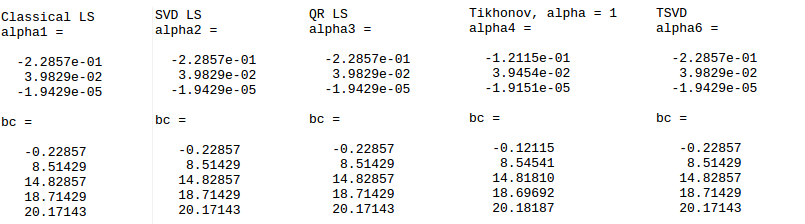
\includegraphics[width=0.7\linewidth]{screenshot013}
\label{fig:screenshot013}
\end{figure}

We need to compare the results according to the error and computation time. Then we choose one of them.
\begin{lstlisting}
Classical LS
	error =  0.67612
	time =  0.049904

SVD LS
	error =  0.67612
	time =  0.71043

QR LS
	error =  0.67612
	time =  0.053302

Tikhonov, alpha = 1
	error =  0.68569
	time =  0.041042

TSVD
	error =  0.67612
	time =  0.44019

General-Cross Validation
	error =  0.68445
	time =  0.045696
\end{lstlisting}

There also was a try to refine the result a little (we choose the classical LS result):
\begin{lstlisting}
x = refinement(A, alpha1, b, 100);
bc = A*x;
disp(["Solution refinement:"])
error = norm(bc - b)
\end{lstlisting}
As it can be seen, after 100 rounds of refinement algorithm, there was not any better solution computed.
\begin{figure}[h]
\centering
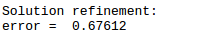
\includegraphics[width=0.45\linewidth]{screenshot015}
\label{fig:screenshot015}
\end{figure}

Therefore the polynomial can be stated as:\\
\begin{math}
y = -0.22857 + 0.039829 x -0.000019429 x^2
\end{math}

The plot of the line described by y is presented on the figure:
\begin{figure}[h]
\centering
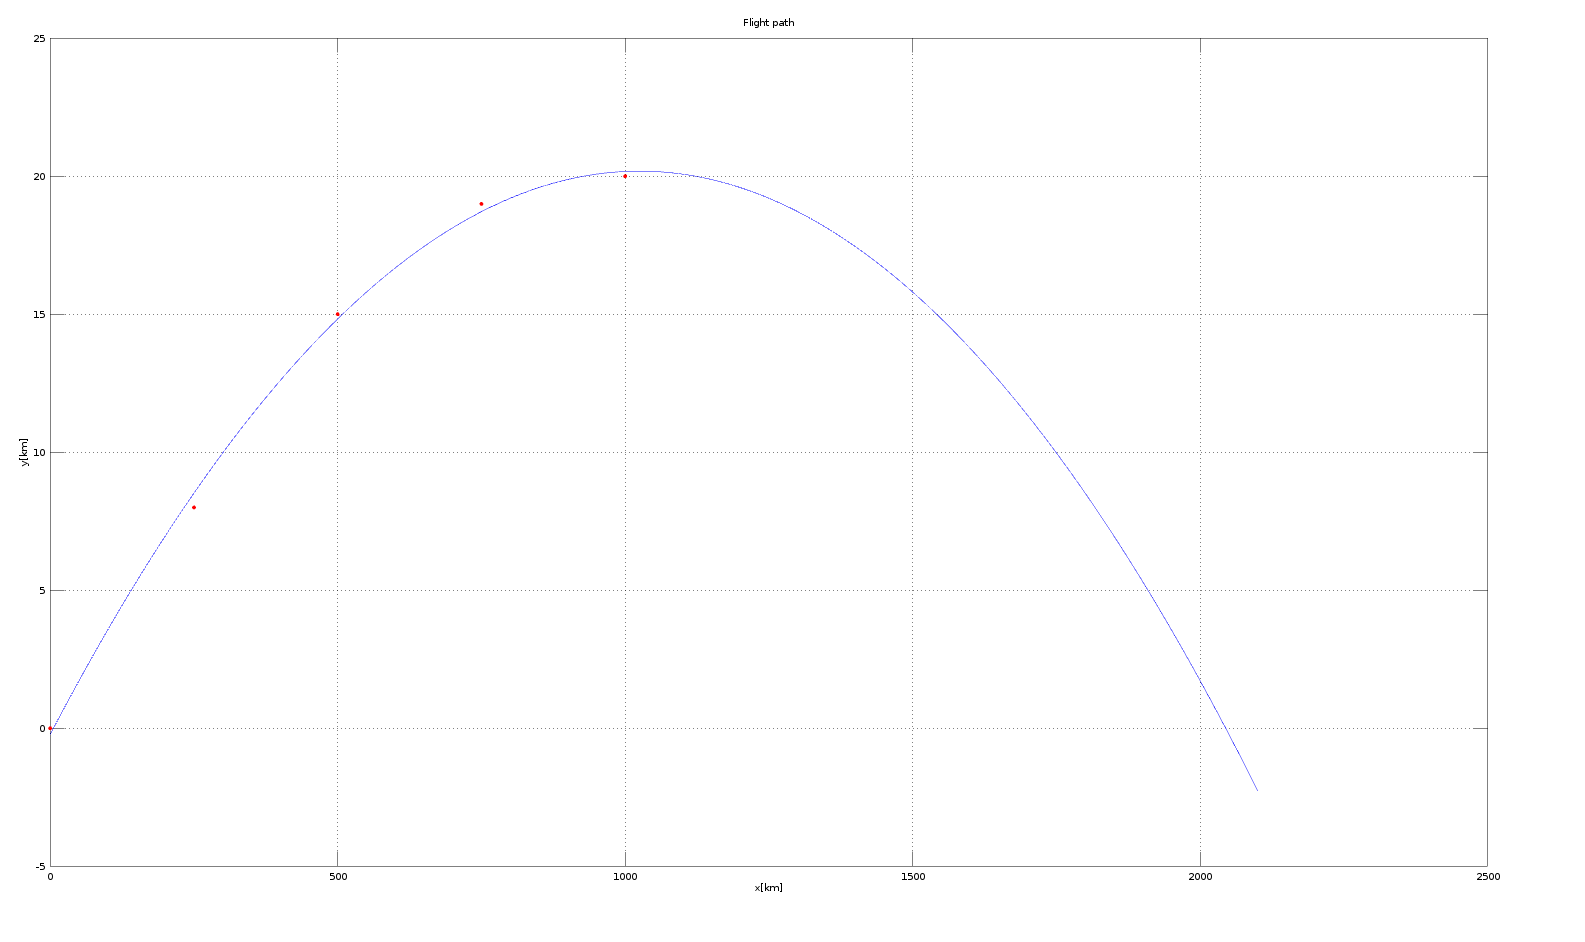
\includegraphics[width=0.7\linewidth]{screenshot016}
\caption{}
\label{fig:screenshot016}
\end{figure}
The rocket should land around 2100 km away from point zero. However, we can check the equation roots to determine the more accurate landing position:
The roots of the presented equation are:\\\\
\begin{math}
x_1 = 5.7550
x_2 = 2044.2450
\end{math}
\\\\According to LS solution, the land-point is around 2044km from point zero.
\newpage

\begin{figure}[h]
\centering
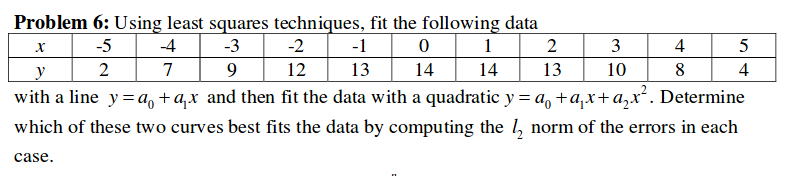
\includegraphics[width=0.7\linewidth]{screenshot017}
\label{fig:screenshot017}
\end{figure}

\begin{figure}[h]
\centering
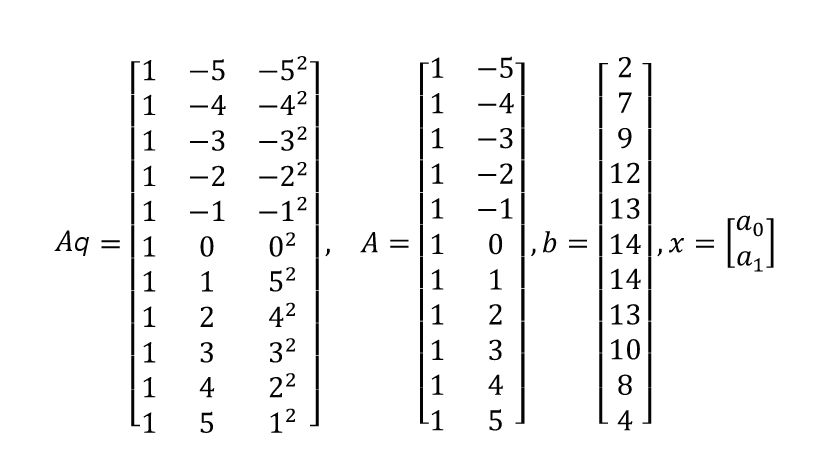
\includegraphics[width=0.4\linewidth]{screenshot018}
\label{fig:screenshot018}
\caption{Task's input data, is presented in the required form - matrices.}
\end{figure}

For the given data, the solutions were calculated for bot line and quadratic functions:
\begin{math}
alpha = \;\;[9.63636 \;\;\;\;0.18182]\\
alphaq = [13.97203 \;\;0.18182 \;\;-0.43357]\\\\
\end{math}
According to results, the functions can be written.\\\\
\begin{math}
y = 0.1818 x + 9.63636 \;\;\;\;\;\;\;\;y_q = -0.43357x^2 + 0.18182x + 13.97203\\\\
L_2
\end{math}
-norms of the errors were also computed, as it was one of the tasks:

\begin{math}
l_{2line} = 12.76 \;\;\;\;\;\;\;\;\;\;\;\;\;\;\;\;\;\;\;\;\;l_{2quad} =  1.27\\
\end{math}
\begin{figure}[h]
\centering
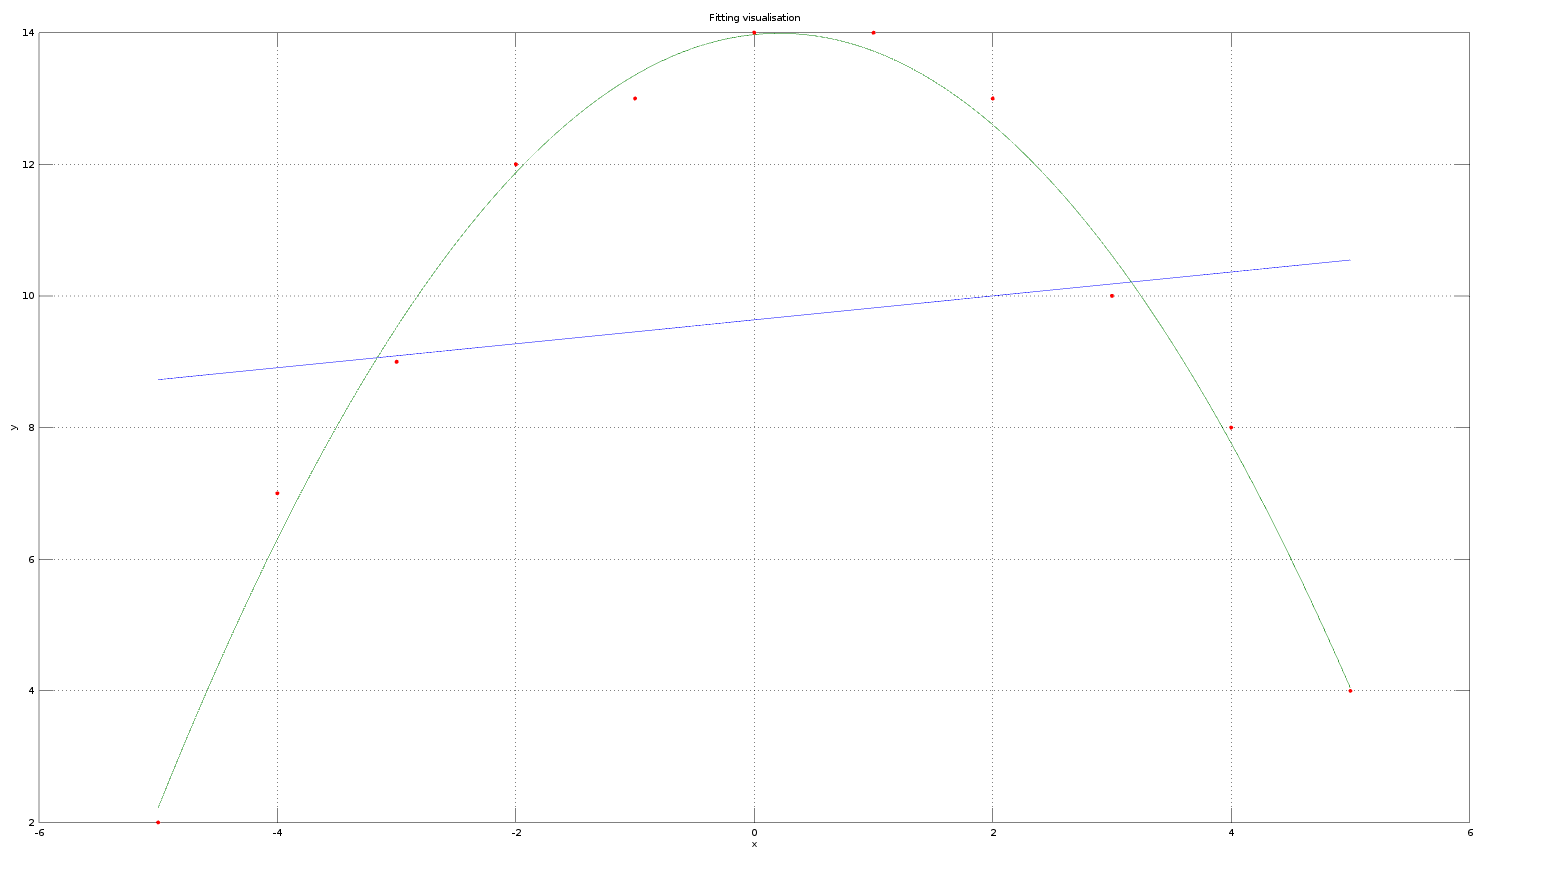
\includegraphics[width=0.9\linewidth]{screenshot020}
\label{fig:screenshot020}
\caption{Final solutions are presented on a plot according to points, line and quadratic function.}
\end{figure}
\newpage
\begin{figure}
\centering
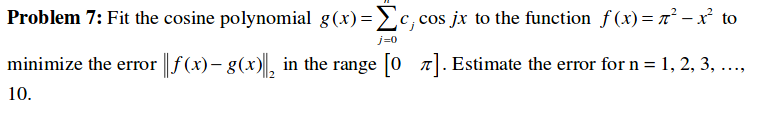
\includegraphics[width=0.7\linewidth]{screenshot021}
\label{fig:screenshot021}
\end{figure}
The following Octave code was prepared to solve the following task:
\begin{lstlisting}
x = 0:0.01:pi;

F = pi.^2 - x.^2;
f = F';

#we assume the largest polynomial
n = 10;
for i = 1:n
G(:,i)=cos(i*x);
endfor

#Ax = b, so to this task GC = f

C = svdLS(G,f)
y = G*C;

plot(x,y, "b", x, f, "r");

grid on
xlabel('x')
ylabel('y')
title('Fitting visualisation')
\end{lstlisting}
\begin{figure}[h]
\centering
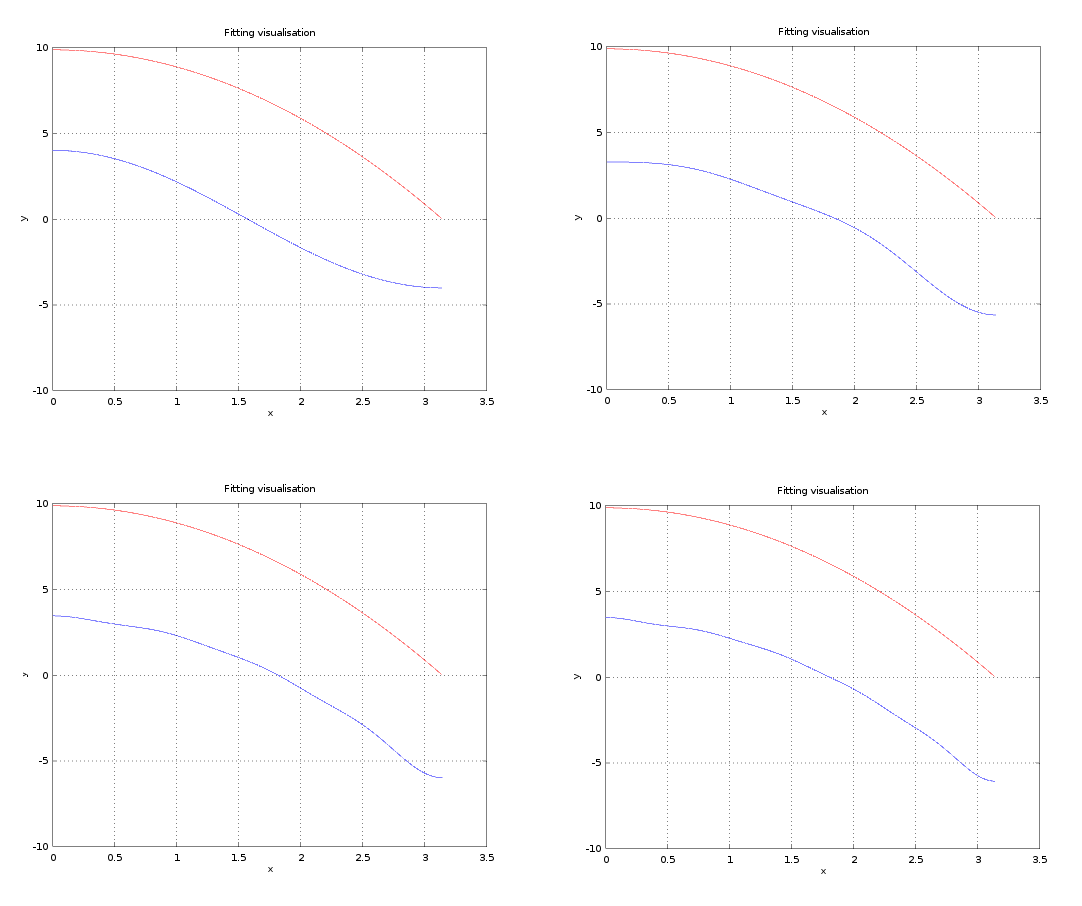
\includegraphics[width=0.7\linewidth]{screenshot022}
\caption{Different line fitting (for N = 1,4,7,10)}
\label{fig:screenshot022}
\end{figure}
\newpage
The error for different n:
\begin{lstlisting}
Error for n = 1
	error =  117.60
Error for n = 2
	error =  116.97
Error for n = 3
	error =  116.83
Error for n = 4
	error =  116.80
Error for n = 5
	error =  116.78
Error for n = 6
	error =  116.78
Error for n = 7
	error =  116.77
Error for n = 8
	error =  116.77
Error for n = 9
	error =  116.77
Error for n = 10
	error =  116.77
\end{lstlisting}

The error does not vary much according to increasing n value, but of course slight change can be observed.\\
\textbf{Line is fitted quite well, but there is certainly a constant missing. However according to g(x) function, we weren't supposed to find a solution including constant value.}
\newpage
\begin{figure}[h]
\centering
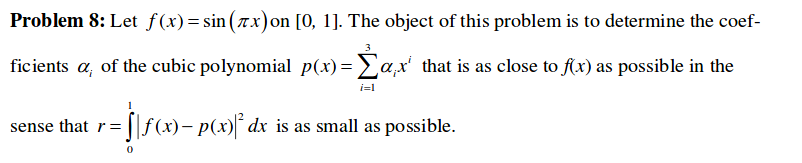
\includegraphics[width=0.7\linewidth]{screenshot023}
\label{fig:screenshot023}
\end{figure}

This task objective is to find the cubic polynomial coefficients to minimize the presented integral.\\
To achieve this, the following file was prepared:
\begin{lstlisting}
#preparing the input data
x = 0:0.1:1;
f = sin(pi*x)';

for i = 1:1:3
p(:,i)=x.^i;
endfor

#different methods
x1 = classicLS(p, f);
x2 = qrLS(p,f);
x3 = svdLS(p,f);
x4 = tikhonovGen(p,f,1);
x5 = tikhonovIt(p,f,100,0.2);
x6 = tsvd(p,f,100);

#calculating the functions according to computed coefficients
Y1 = p.*x1'
Y2 = p.*x2'
Y3 = p.*x3'
Y4 = p.*x4'
Y5 = p.*x5'
Y6 = p.*x6'

#minimizing condition
integral1 = quad(@(x)fun(x,Y1),0,1)
integral2 = quad(@(x)fun(x,Y2),0,1)
integral3 = quad(@(x)fun(x,Y3),0,1)
integral4 = quad(@(x)fun(x,Y4),0,1)
integral5 = quad(@(x)fun(x,Y5),0,1)
integral6 = quad(@(x)fun(x,Y6),0,1)
\end{lstlisting}
\newpage
And the following results were obtained:
\begin{figure}[h]
\centering
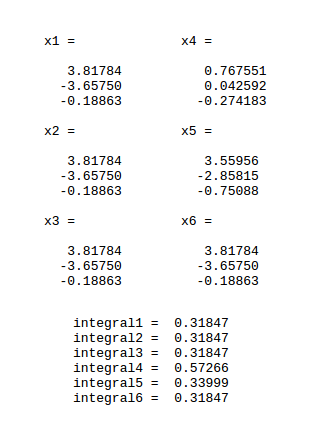
\includegraphics[width=0.5\linewidth]{screenshot024}
\label{fig:screenshot024}
\end{figure}

As it can be seen, the results of every method beside Tikhonov-based, are the same. In case of their equivalence, also the error will be just the same.
\newpage
\begin{figure}[h]
\centering
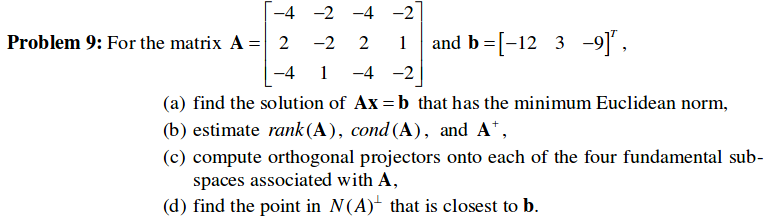
\includegraphics[width=0.7\linewidth]{screenshot025}
\label{fig:screenshot025}
\end{figure}
The following code was designed to solve task no. :
\begin{lstlisting}
A = [-4 -2 -4 -2; 2 -2 2 1; -4 1 -4 -2]
b = [-12; 3; 9]

#Task a)
#x1 = classicLS(A,b)
#x2 = qrLS(A,b)
x3 = svdLS(A,b)
x4 = tikhonovGen(A,b,1)
x5 = tikhonovIt(A,b,100,0.2)
x6 = tsvd(A,b,100)

#n1 and n2 cannot be used because of precision
#n1 = norm(A*x1 - b,2)
#n2 = norm(A*x2 - b,2)
n3 = norm(A*x3 - b,2)
n4 = norm(A*x4 - b,2)
n5 = norm(A*x5 - b,2)
n6 = norm(A*x6 - b,2)

#Task b)
rref(A)
rank(A)
Aplus = pseudoinverse(A)

#Task c)
[Pra, Prah, Pna, Pnah] = projectors(A)
\end{lstlisting}

Calculations of the LS and the norm of the solution:\begin{figure}[h]
\centering
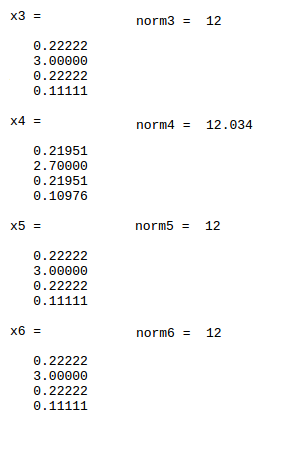
\includegraphics[width=0.3\linewidth]{screenshot026}

\label{fig:screenshot026}
\end{figure}

According to the RREF, the matrix looks like that:
\begin{figure}[h]
\centering
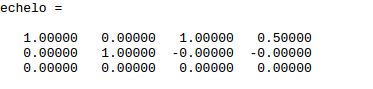
\includegraphics[width=0.4\linewidth]{screenshot027}
\caption{RREF of matrix A.}
\label{fig:screenshot027}
\end{figure}

As the figure can idicate, the matrix rank should be equal to 2 (which is exactly the answer compiuted by Octave).
\\
\\
We were also requested to compute the pseudoinverse of Matrix A and its orthonormal projectors:
\begin{figure}[h]
\centering
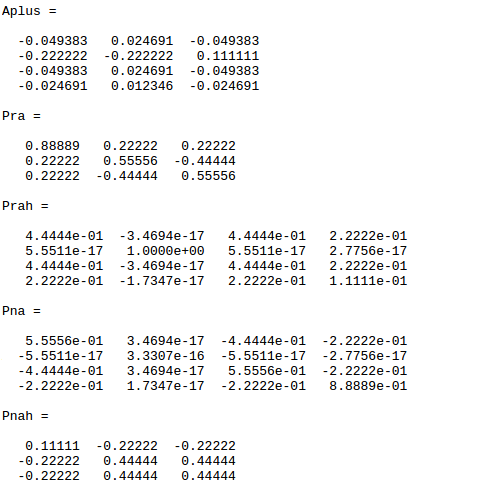
\includegraphics[width=0.7\linewidth]{screenshot028}
\label{fig:screenshot028}
\end{figure}
\newpage
\begin{figure}[h]
\centering
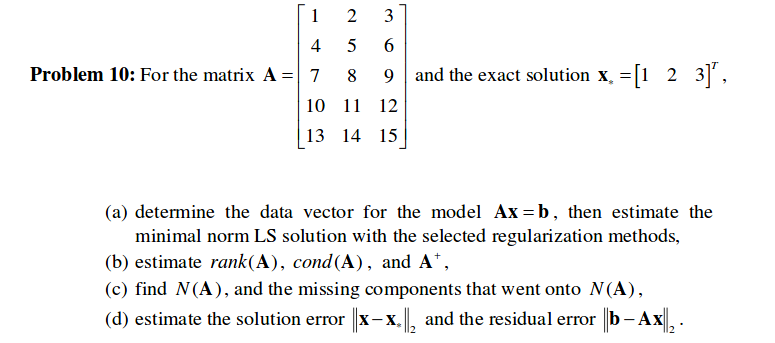
\includegraphics[width=0.7\linewidth]{screenshot029}
\label{fig:screenshot029}
\end{figure}
The following code was prepared to solve all the requested tasks:
\begin{lstlisting}
A = [1 2 3; 4 5 6; 7 8 9; 10 11 12; 13 14 15]
x_exact = [1 2 3]'
b = A*x_exact

x1 = tsvd(A,b,1000)
x2 = tikhonovIt(A,b,1000,0.1)

Echelon = rref(A)
RankA = rank(A)
APlus = pseudoinverse(A)

error1 = sum((x1-x_exact).^2)
Rerror1 = sum((b-A*x1).^2)
error2 = sum((x2-x_exact).^2)
Rerror2 = sum((b-A*x2).^2)
\end{lstlisting}
\begin{figure}[h]
\centering
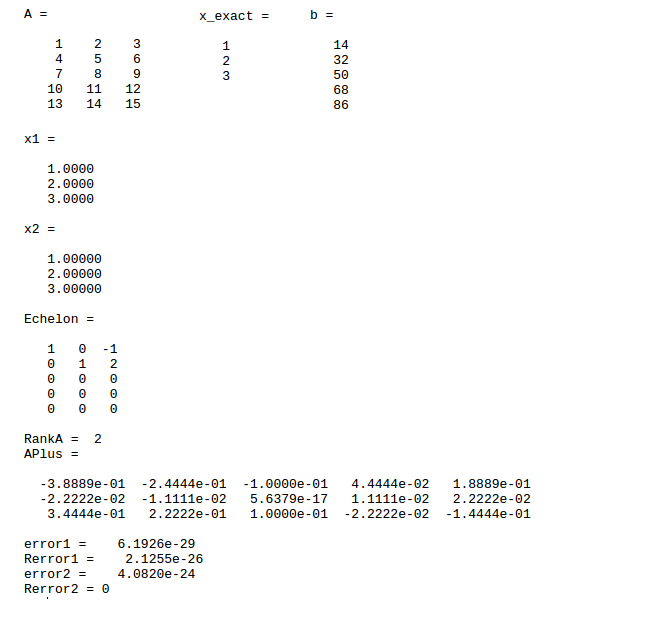
\includegraphics[width=0.7\linewidth]{screenshot030}
\label{fig:screenshot030}
\end{figure}

During computations we obtained exact solution, so all the errors are a result of computer arithmetic and numbers rounding.
\newpage

\begin{figure}[h]
\centering
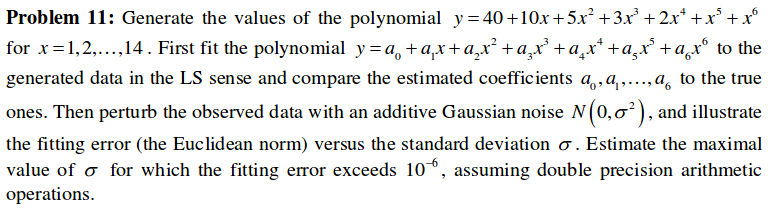
\includegraphics[width=0.7\linewidth]{screenshot031}
\label{fig:screenshot031}
\end{figure}
\begin{lstlisting}
a=[40; 10; 5; 3; 2; 1; 1];

%Coefficients
x=1:1:14;
X = x';
A = [X.^0 X.^1 X.^2 X.^3 X.^4 X.^5 X.^6];
%sample x values
y=40+10*x+5*x.^2+3*x.^3+2*x.^4+x.^5+x.^6;

C = tsvd(A,y',10)
C_exact = A\y'
\end{lstlisting}
\begin{figure}[h]
\centering
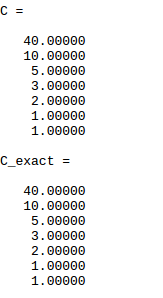
\includegraphics[width=0.2\linewidth]{screenshot032}
\caption{Using computations the solution that corresponds to exact coefficients was obtained.}
\label{fig:screenshot032}
\end{figure}
\newpage
\begin{figure}[h]
\centering
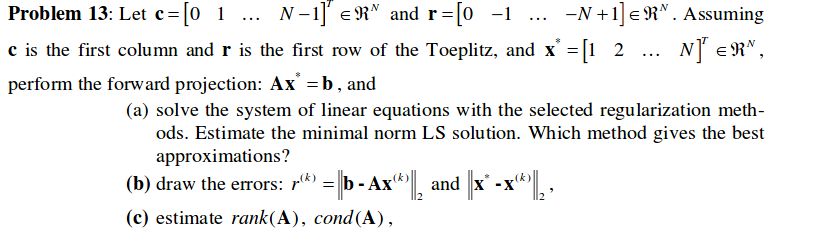
\includegraphics[width=0.6\linewidth]{screenshot034}

\label{fig:screenshot034}
\end{figure}

\begin{figure}[h]
\centering
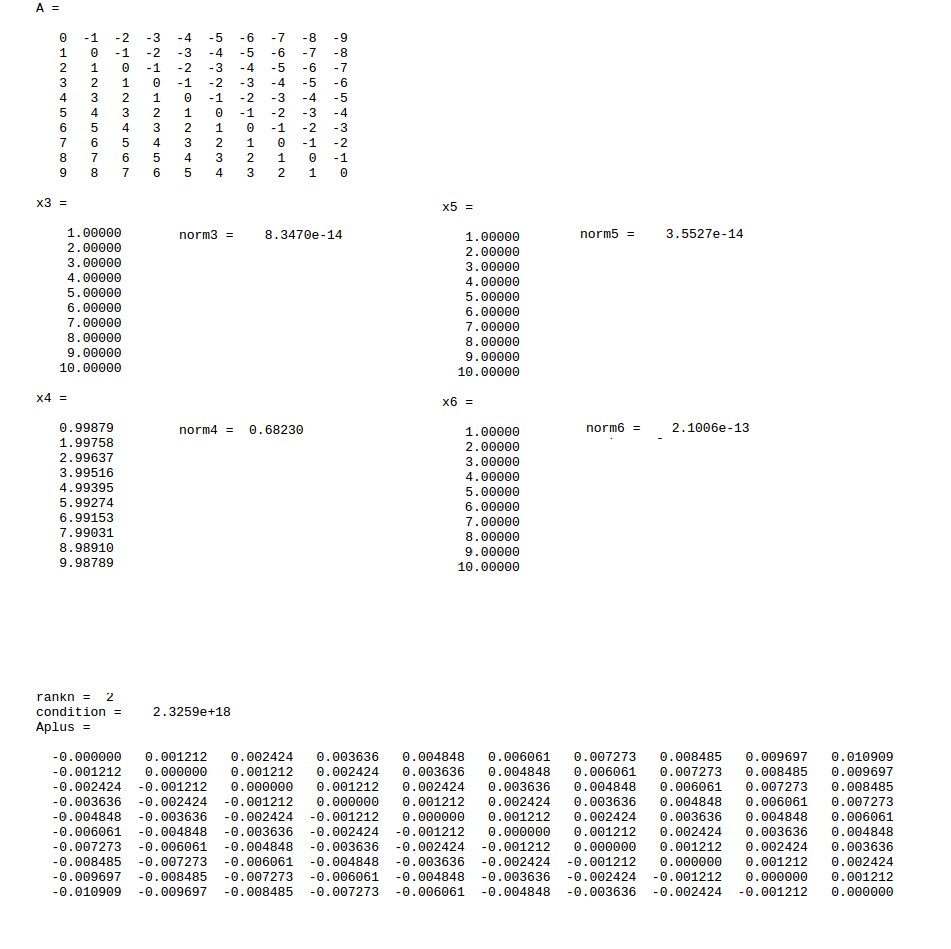
\includegraphics[width=0.9\linewidth]{screenshot033}
\caption{(Norm on the image are the l2 norm calculated from errors.)}
\label{fig:screenshot033}
\end{figure}















\chapter{Algorithms code}
Algorithm \space 1 -- The classical LS fitting.\\
\begin{lstlisting}
function [x] = classicLS(A, b)

[m,n] = size(A)

if(m >= n || rank(A) == n)
	disp(["There is an unique solution"])
	x = inv(A' * A) * A' * b;
else if ( m < n)
	disp(["Underdetermined system"])
	x = A' * inv(A * A') * b;
end
endfunction
\end{lstlisting}


Algorithm \space 2 -- Pseudoinverse\\
\begin{lstlisting}
function [x] = pseudoinverse(A)

[m,n] = size(A);
r = rank(A);
[u,s,v] = svdqr(A,20);

x = zeros(n,m);

for i = 1:r
	x = x + inv(s(i,i)) *v(:,i)* u(:,i)';
endfor

endfunction
\end{lstlisting}
\newpage
Algorithm \space 3 -- The orthogonal projectors\\
\begin{lstlisting}
function [Pra, Prah, Pna, Pnah] = projectors(A)

[m,n] = size(A)

Pra = A * pseudoinverse(A)
Prah = pseudoinverse(A) * A

Pnah = eye(size(Pra)) - Pra
Pna = eye(size(Prah)) - Prah

endfunction
\end{lstlisting}

Algorithm \space 4 -- The LS solution by SVD\\

\begin{lstlisting}
function [x] = svdLS(A,b)

[u,s,v] = svd(A);

x = (v*pseudoinverse(s) * u') * b;

endfunctiong
\end{lstlisting}
Algorithm \space 5 -- The LS solution by QR factorization\\
\begin{lstlisting}
function [U, S, V] = svdQR(A,iterations)

[n, m]= size(A); # can be rectangular matrix
U=eye(n);   
V=eye(m);

R=A';  

for i = 0:iterations
	[Q,R]=qr(R');   # qr decompositions and updating  
	U=U*Q;         
	[Q,R]=qr(R');
	V=V*Q;
endfor
S=R';               # S is R transposed

endfunction
\end{lstlisting}
\newpage
Algorithm \space 6 -- The linear regression\\
\begin{lstlisting}
function [x] = regression(A, b)

[m,n] = size(A
[p,r] = size(b);

if(n != 2 || r != 1)
	disp(["The matrix does not describe the polynomial of first degree"])

else
	meanY = sum(b)/p
	meanT = sum(A(:,n))/m
	
	#beta = (sum(b.*A(:,n)) - m*meanY*meanT)/(sum(A(:,n).^2) - m * meanT*meanT)
	#alpha = meanY - beta*meanT
	
	#more accurate b calculation
	first = (b.- meanY).*(A(:,n).-meanT)
	second = (b.-meanT).^2
	beta = sum(first)/sum(second)
	alpha = meanY - beta*meanT
	
	x = [alpha;beta]
endif
endfunction
\end{lstlisting}
Algorithm \space 7 -- The TSVD algorithm\\
\begin{lstlisting}
function [x] = tsvd(A,b, it)

[u,s,v] = svdqr(A,it);

c = u'*b
r = rank(A)
x=zeros(size(A,2),1);

for i = 1:r
	x = x + (c(i)*v(:,i))/s(i,i);
endfor
endfunction
\end{lstlisting}
Algorithm \space 8 -- The iterative refinement\\
\begin{lstlisting}
function [x] = refinement(A,x,b,it)

for s = 1:it
	r = b - A*x
	
	#extended refinement
	delta = qrLS(A,r);
	x = x + delta
endfor
endfunction
\end{lstlisting}
Algorithm 10 -- The General Cross-Validation\\
\begin{lstlisting}
function [x] = crossvalidation(A,b, mi)

C = inv(A'*A);
M = A' * A + (mi.^2).^C'*C;

x = inv(M)*A'*b;

endfunction
\end{lstlisting}
Algorithm 11 -- The Iterative Tikhonov Regularization\\
\begin{lstlisting}
function [x] = tikhonovIt(A,b, it, mi)

[m,n] = size(A);

x=zeros(size(A,2),1);
for i = 1:it
	x = x + inv(A' * A + eye(size(A'*A)).*mi) * A' * (b-A*x);
endfor

endfunction
\end{lstlisting}
Algorithm ** -- The General Tikhonov Regularization\\
\begin{lstlisting}
function [x] = tikhonovGen(A,b, alpha)

x = inv(A' * A + alpha.*eye(size(A'*A))) * A' * b;

endfunction
\end{lstlisting}
\begin{thebibliography}{8}
\addcontentsline{toc}{chapter}{Bibliography}
%\addcontentsline{toc}{section}{Literatura}
\bibitem{bjorck}
Björck, Åke. Numerical methods for least squares problems. Society for Industrial and Applied Mathematics, 1996.
\bibitem{meyer} 
C. D. Meyer, Matrix Analysis and Applied Linear Algebra, SIAM, 2000, 
\bibitem{zarowski}
Ch. Zarowski, An Introduction to Numerical Analysis for Electrical and Computer Engineers, Wiley, 2004
\bibitem{zdunek}
Zdunek R., Numerical Methods - lecture slides.
\end{thebibliography}

\end{document}

